\documentclass[12pt,letterpaper]{article}
\usepackage[top=0.85in,left=1in,footskip=0.75in,marginparwidth=2in]{geometry}

% use Unicode characters - try changing the option if you run into troubles with special characters (e.g. umlauts)
\usepackage[utf8]{inputenc}

% clean citations
\usepackage{cite}

% hyperref makes references clicky. use \url{www.example.com} or \href{www.example.com}{description} to add a clicky url
\usepackage{nameref,hyperref}

% line numbers
\usepackage[right]{lineno}

% improves typesetting in LaTeX
\usepackage{microtype}
\DisableLigatures[f]{encoding = *, family = * }

% text layout - change as needed
\raggedright
\setlength{\parindent}{0.5cm}
\textwidth 6.5in 
\textheight 9in
\renewcommand{\baselinestretch}{1.5}

% use adjustwidth environment to exceed text width (see examples in text)
\usepackage{changepage}

% adjust caption style
\usepackage[font=small,aboveskip=1pt,labelfont=bf,labelsep=period,singlelinecheck=off]{caption}

% remove brackets from references
\makeatletter
\renewcommand{\@biblabel}[1]{\quad#1.}
\makeatother

% headrule, footrule and page numbers
\usepackage{lastpage,fancyhdr,graphicx}
\usepackage{epstopdf}
\pagestyle{myheadings}
\pagestyle{fancy}
\fancyhf{}
\rfoot{\thepage/\pageref{LastPage}}
\renewcommand{\footrule}{\hrule height 2pt \vspace{2mm}}
\fancyheadoffset[L]{2.25in}
\fancyfootoffset[L]{2.25in}

% use \textcolor{color}{text} for colored text (e.g. highlight to-do areas)
\usepackage{color}

% define custom colors (this one is for figure captions)
\definecolor{Gray}{gray}{.25}

% this is required to include graphics
\usepackage{graphicx}
\usepackage{subcaption}
\usepackage{pdflscape}
\graphicspath{{../figures/}}

% use if you want to put caption to the side of the figure - see example in text
\usepackage{sidecap}

% use for have text wrap around figures
\usepackage{wrapfig}
\usepackage[pscoord]{eso-pic}
\usepackage[fulladjust]{marginnote}
\reversemarginpar
\usepackage{amsmath}

% document begins here
\begin{document}
\vspace*{0.35in}

% title goes here:
\begin{flushleft}
{\Large
\textbf\newline{Title}
}
\newline
% authors go here:
\\
%Fatemeh Ashari Ghomi\textsuperscript{1},
%Paul P. Gardner\textsuperscript{1,*},
%Lars Barquist\textsuperscript{2}
%\\
%\bigskip
%\bf{1} University of Canterbury
%\\
%\bf{2} Wurzburg University
%\\
%\bigskip
%* paul.gardner@canterbury.ac.nz

\end{flushleft}

\section*{Abstract}
%Many genes have been identified with advances in sequencing technology and genome annotation methods. However, not all of these genes are of the same importance. We have used transposon mutagenesis to investigate gene essentiality in 14 strains of Enterobacteriaceae. We investigated the potential biases of this approach and found an origin of replication bis, no preferred insertion motif bias, a G-C bias in low G-C genes,  and positional bias within genes. After correcting for these biases, we investigated the changes in the cohorts of essential genes and compared them to their conservation level. Surprisingly, we found that conserved genes are not necessarily essential, and essential genes are not necessarily conserved. However, on average, essential genes are more likely to be conserved.

% now start line numbers
\linenumbers

% the * after section prevents numbering
\section{Introduction}
%The study of cells can give us new insights for understanding the foundation of life. However, the naturally existing cells are very complex which hampers the study of their constituents. Restricting these studies to the genes that are required for the growth of cells can reduce this complexity and enable us to study life in its simplest form \cite{juhas_essence_2011}.

Generating genomic variants that carry genes responsible for essential cellular processes can open up new research directions. Adding genes or metabolic pathways to cells provides new variants with specialised phenotypes. Modified cells have different potential applications in biotechnology \cite{juhas_bacillus_2014}, fuel production \cite{seo_synthetic_2013}, healthcare, and food production \cite{juhas_meeting_2013}. Another important application for studying essential genes is in drug discovery \cite{juhas_essential_2012}. Infectious diseases are among the top major causes of mortality worldwide. Even though antibiotic resistance is growing among bacteria, the antibiotic discovery and development rate is diminishing \cite{fischbach_antibiotics_2009, nathan_antibiotics_2004}. Therefore, it is urgent to find new drugs for infectious diseases. New antibiotics target genes that are essential for the survival of pathogenic bacteria in order to control disease. Some well-known antibiotics that target essential functions are tetracyclines that bind to small ribosomal subunit and interfere with protein translation \cite{brodersen_structural_2000}, penicillins that target peptidoglycan and inhibit the cell wall synthesis \cite{chung_rapid_2009}, and quinolones that target DNA Gyrase \cite{marcusson_interplay_2009}.
%Some candidate antibiotic targets found by investigating essential genes are trans-translation genes \textit{ssrA} and \textit{smpB} from \textit{helicobacter pylori} \cite{thibonnier_trans-translation_2008}, \textit{CcrM} and \textit{MenH} which are bacterial methyltransferases, and \textit{lptD} (previously known as \textit{ostA}) in \textit{Pseudomonas aeruginosa} \cite{srinivas_peptidomimetic_2010} whose essential role is yet under investigation \cite{werneburg_inhibition_2012}.[SOME ANTIBIOTICS THAT TARGET ESSENTIAL GENES ARE...]

In the earliest attempt for the identification of essential genes, Mushegian and Koonin compared the genomes of \textit{Haemophilus influenzae} and \textit{Mycoplasma genitalium}, assuming that the genes that are shared in these two phylogenetically distant bacteria are indispensable and reported 256 genes fulfilling this requirement \cite{mushegian_minimal_1996}. With the advent of sequencing technologies and availability of more genome sequences, the number of core genes in different prokaryotic genomes declined to less than 50 which is not enough for performing all essential functions in a cell \cite{charlebois_computing_2004}. Therefore, the use of experimental methods for the identification of essential genes is vital. Researchers have now studied the essential genes in organisms from all three domains of life \cite{luo_deg_2014} using a number of different methods. Baba et al.\@ \cite{baba_construction_2006} made a library of single gene deletions for \textit{Escherichia coli} K-12. The 303 genes where viable \textit{Escherichia coli} colonies failed to grow are the candidate essential genes. Another group used an antisense RNA knockdown approach to study gene essentiality in \textit{Staphylococcus} aureus \cite{forsyth_genome-wide_2002}. In this method, if the expression of an antisense RNA hinders the growth of the cell, its cognate gene is known as essential. Both of these methods are labour intensive and are dependent on the accuracy of genome annotations. Another widely used procedure is transposon mutagenesis combined with high-throughput sequencing \cite{chao_design_2016, van_opijnen_transposon_2013, barquist_approaches_2013} which includes different approaches namely, Tn-Seq \cite{van_opijnen_tn-seq:_2009}, INSeq \cite{goodman_identifying_2009}, HITS \cite{gawronski_tracking_2009} and TraDIS \cite{langridge_simultaneous_2009}. These procedures differ in the type of transposon, sample preparation methods, and data analysis \cite{van_opijnen_transposon_2013}. Nonetheless, all share the same workflow: pools of single insertion mutants are constructed using transposon mutagenesis. After a growth phase, mutants that are fitter outnumber the less fit ones. Using high-throughput sequencing and tallying transposon junctions gives an indication of whether a genomic region is essential or not. A high number of transposon insertions in a gene indicates that the gene is not essential in its growth medium and conversely, a low number of transposon insertions indicates that a gene is essential in the medium.

There are two groups of essential genes: core essential genes are indispensable for all cells, and accessory essential genes that are required for some organisms. Core essential genes can shed light on the genome structure of the last universal common ancestor and the evolution of living cells \cite{koonin_comparative_2003} and have been used for the synthesis of minimal cells \cite{hutchison_design_2016}. On the other hand, accessory essential genes are helpful in the study of specific lineages. Accessory essential genes may be useful in species-specific antibiotic discovery. Antibiotics that target core essential genes in pathogens may not be ideal, as they may attack homologous genes in their hosts or commensal bacteria.

%Curtis and Brun \cite{curtis_identification_2014} have studied the essentiality changes in cell cycle genes of three alpha-proteobacteria strains: \textit{Caulobacter crescentus}, \textit{Brevundimonas subvibrioides}, and \textit{Agrobacterium tumefaciens} and concluded that although essential genes responsible for cell functions are conserved, there are many essential genes that are specific to each organism.
Freed et al. \cite{freed_combining_2016} have investigated the difference between essential genes in \textit{Shigella flexneri} 2a 2457T and \textit{Escherichia coli} K12 BW25113 and shown that there are no genes that are essential in \textit{Escherichi coli} and not essential in \textit{Shigella flexneri}, while some genes are only essential in \textit{Shigella flexneri}. These include a group of genes involved in cysteine, proline and sugar nucleotide biosynthesis, acetate utilisation, translation elongation, aminoacyl tRNA synthetase, murein DD-endopeptidase, and soxR-reducing complex, many of which are essential in \textit{Shigella flexneri} due to the absence of paralogs or other alternative systems that exist in \textit{Escherichia coli}.
%The difference in essentiality stems from four reasons: the disruption of many of the genes in \textit{Shigella flexneri} 2a 2457T impede the growth, but these genes are not actually essential; the conditions were different in the two experiments done on \textit{Escherichia coli} K12 BW25113 and \textit{Shigella flexneri} 2a 2457T; many of the genes were not actually essential for growth, but essential for transposon insertion and antibiotic resistance; and

%PPG: Reduce, summarise main findings of Canals & Barquist. e.g. Most essential genes are also essential in related species, yet there are some serovar-specific essential genes [GIVE SOME NUMBERS]... 
Canals et al.\@ \cite{canals_high-throughput_2012} have compared the essentiality of genes in \textit{Salmonella} typhimurium ATCC 14028, two isolates of \textit{Salmonella typhi} Ty2 (varying in \textit{htrA}, \textit{aroC} and \textit{aroD} genes), and \textit{Escherichia coli} K12 BW25113 and found that these cells share 268 essential genes. Nine genes are essential in \textit{Escherichia coli} and not essential in \textit{Salmonella}s, three of which can tolerate insertions only in some parts and one has distant paralogs in \textit{Salmonella}s that is missing in \textit{Escherichia coli}. For other genes, there are a few insertions in \textit{Salmonella}s, but the number is not small enough to call those genes essential. Moreover, 159 genes were almost essential in all \textit{Salmonella}s but not in \textit{Escherichia coli}. These include genes involved in replication and genes related to ribosome and its accessory proteins. The authors also found 26 genes that are under greater selection in \textit{Salmonella} Typhimurium compared to \textit{S. typhi} and 10 genes vice versa. Barquist et al. \cite{barquist_comparison_2013} have used transposon-directed insertion-site sequencing to compare the essentiality of genes in \textit{Salmonella} Typhi Ty2, \textit{Salmonella} Typhimurium SL1344, and \textit{Escherichia coli} K12 BW25113. 
%THIS IS IMPORTANT:
These genomes share 228 essential genes which are mostly involved in cell division, transcription, translation, and fatty acid and peptidoglycan biosynthesis. Additionally, many of the serovar-specific essential genes in \textit{Salmonella}s are phage repressors. Another key difference between these two serovars is that a set of genes that are putatively involved in cell wall biosynthesis are essential in \textit{Salmonella} Typhimurium and not essential in \textit{salmonella} Typhi which gives an indication of the adaptation of these two \textit{Salmonella} serovars to their niches.

Although there are some studies on differentiation of essentiality in different organisms, these studies usually include a few genomes. We are going to extend these studies to a larger scale in Enterobacteriaceae family. Our aim is to study the essentiality of genes in in 16 different organisms. These include \textit{Enterobacter cloacae} NCTC 9394, \textit{Klebsiella pneumoniae} Ecl8, \textit{Klebsiella pneumoniae} RH201207, \textit{Citrobacter rodentium} ICC168, \textit{Salmonella} Typhimurium SL1344, \textit{Salmonella} Typhimurium SL3261, \textit{Salmonella} Typhimurium D23580, \textit{Salmonella} Typhimurium A130, \textit{Salmonella} Enteritidis P125109, \textit{Salmonella} Typhi Ty2, \textit{Escherichia coli} ST131 EC958, \textit{Escherichia coli} UPEC ST131, \textit{Escherichia coli} ETEC CS17, \textit{Escherichia coli} ETEC H10407, \textit{Escherichia coli} BW25113, and \textit{Escherichia coli} K-12 MG1655.

%WHAT FATEMEH DID....

%Enterobacteriaceae is a well characterised family of Gram-negative bacteria with a variety of host ranges and pathogenecity \cite{brenner_bergeys_2006}. In addition, we added the essential genes of \textit{Escherichia coli} K-12 MG1655 from EcoGene database \cite{zhou_ecogene_2013} to our study. In EcoGene the essentiality of genes suggested as essential by Baba et al.\@ \cite{baba_construction_2006} has been further studied and only 299 out of 303 genes are marked as essential. We first performed a detailed study of biases than can influence the inference of essentiality. Then, we normalised our data for the biases and investigated the essentiality of genes in three classes of genes: genus specific (genes that are present only in one genus), single copy genes (genes with about one instance per genome in all of the genomes that we are studying), and multi-copy genes(genes that are copied multiple times per genome). We have also investigated how essentiality changes in the phylogenetic tree for these organisms.

%\begin{figure}
%\includegraphics[scale=0.2]{phylosift-aa-raxmlbootstrap.pdf}
%\caption{The species tree containing the 16 genomes used in this study. We have generated the tree by running RAxML \cite{stamatakis_raxml_2014} on Phylosift \cite{darling_phylosift:_2014} amino acid markers.}
%\label{fig:species-tree}
%\end{figure}

\section{Results and Discussion}
\subsection{Incorporating multiple measures of gene essentiality improves prediction}
In this section we will compare a number of methods of quantifying the essentiality of genes based on transposon insertion data and introduce our own method.
\subsubsection{Comparison of old methods}
A number of methods have been used for evaluating the essentiality of genes using transposon insertion data. Freed et al. \cite{freed_combining_2016} have compared eleven features that can quantify the essentiality of genes. These include: the number of insertion sites within genes; the mean distance between insertion sites, the median distance between insertion sites, the number of base pairs before the first insertion in the $5^\prime$ end, the ratio between the number of base pairs before the first insertion in the $5^\prime$ end and gene length, the number of base pairs before the second insertion in the $5^\prime$ end, the ratio between the number of base pairs before the second insertion in the $5^\prime$ end and gene length, the length of the longest uninterrupted region in the gene, the ratio between the length of the longest uninterrupted region in the gene and gene length, the length of the longest region in the gene containing at most one insertion divided by gene length, and the number of insertion sites divided by gene length. Among these, the average distance between insertion sites and the length of the longest uninterrupted region were the best predictors.

Barquist et al. \cite{barquist_tradis_2016} have used insertion indices which are calculated by dividing the number of insertion sites by gene length for defining the essentiality of genes. Plotting all insertion indices for all genes in a genome gives a bimodal plot, each mode representing a group of genes (essential or non-essential). They have fitted two gamma distributions to these modes and calculated the log odds value for each gene to test which mode it belongs to.

Turner et al. \cite{turner_essential_2015} have randomly sampled insertions in a genome and using DESeq package \cite{anders_differential_2010} calculated log fold changes and P-values for the actual number of insertions compared to the expected number of insertions obtained from the sampling method.

We have compared the predictive power of the average distance between insertion sites in a gene, the length of the longest uninterrupted region, insertion index, log odds value obtained from insertion index value, and P-value and log fold change calculated using DESeq package after sampling. To evaluate the accuracy of these methods, we have compared the predicted essential genes to the essential genes in \textit{Escherichia coli} K-12 MG1655 in EcoGene database \cite{zhou_ecogene_2013}. The results are depicted in Figure~\ref{fig:benchmark}. Among all methods, those that try to fit a distribution to data and predict essentiality based on that, namely log odds value from insertion indices and P-value from DESeq after sampling, are the least accurate methods. Sampling and then calculating log fold changes using DESeq package is the most accurate predictor and the other three methods are also good predictors despite their simplicity.
\subsubsection{PCA based method}\label{sec:essentiality-call}
We selected four of the predictors in previous section: insertion index, log fold change using sampling and DESeq, the average distance between insertion sites in a gene, and the length of the longest uninterrupted region. These predictors were selected as they were more accurate and less dependent on each other. Afterwards, we ran principal component analysis on these predictors using \emph{prcomp} function in R and selected the first principal component. As Figure~\ref{fig:benchmark} shows, PCA results gave us the most powerful tool for quantifying the essentiality of genes compared to other methods. We have plotted the results for one sample genome and the results for other genomes are shown in {\color{red}SUPPLEMENTARY}. Figure~\ref{fig:pca} shows the distribution of PCA results after zero mean unit variance normalisation. We call this value NPEQ (Normalised Pca based Essentiality Quantifier) in this paper. The genes whose NPEQ values are less than -1.644854 after normalisation are beneficial losses and the genes with NPEQ greater than 1.644854 are essential. The rest are non-essential genes. The cutoff 1.644854 has been selected because if we assume that NPEQ distribution is normal, this cutoff shows the P-value 0.95. Moreover, by trying to define a cutoff that maximises Matthews correlation coefficient for each genome using NPEQ, we get 1.650449 as the average cutoff which is very close to this value.

\begin{figure}
\captionsetup[subfigure]{justification=centering}
\begin{subfigure}{.5\textwidth}
  \centering
  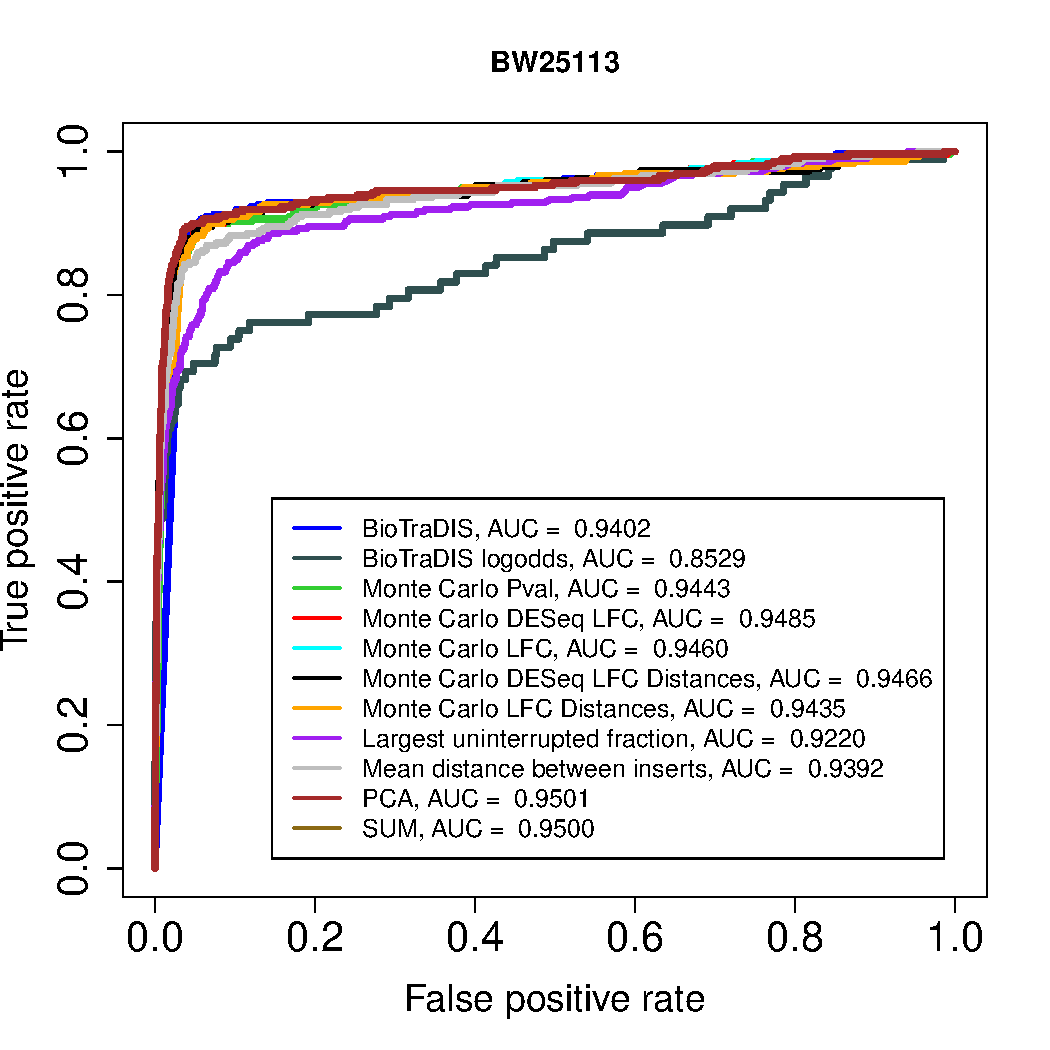
\includegraphics[page=1, scale=0.4]{essential-call-comparison-BW25113.pdf}
  \caption{}
  \label{fig:benchmark}
\end{subfigure}%
\begin{subfigure}{.5\textwidth}
  \centering
  \includegraphics[page=10, scale=0.4]{essential-call-comparison-BW25113.pdf}
  \caption{}
  \label{fig:pca}
\end{subfigure}
\caption{(a) The accuracy of 7 different prediction methods for quantifying the essentiality of genes. The higher the area under the curve, the more accurate the method is. (b) The distribution for our proposed method (NPEQ)}
\label{fig:essentiality-call}
\end{figure}

%\begin{figure*}
%\centering
%\begin{tabular}{c c c}
%\includegraphics[page=1, scale=0.23]{essential-call-comparison-BN373.pdf}&
%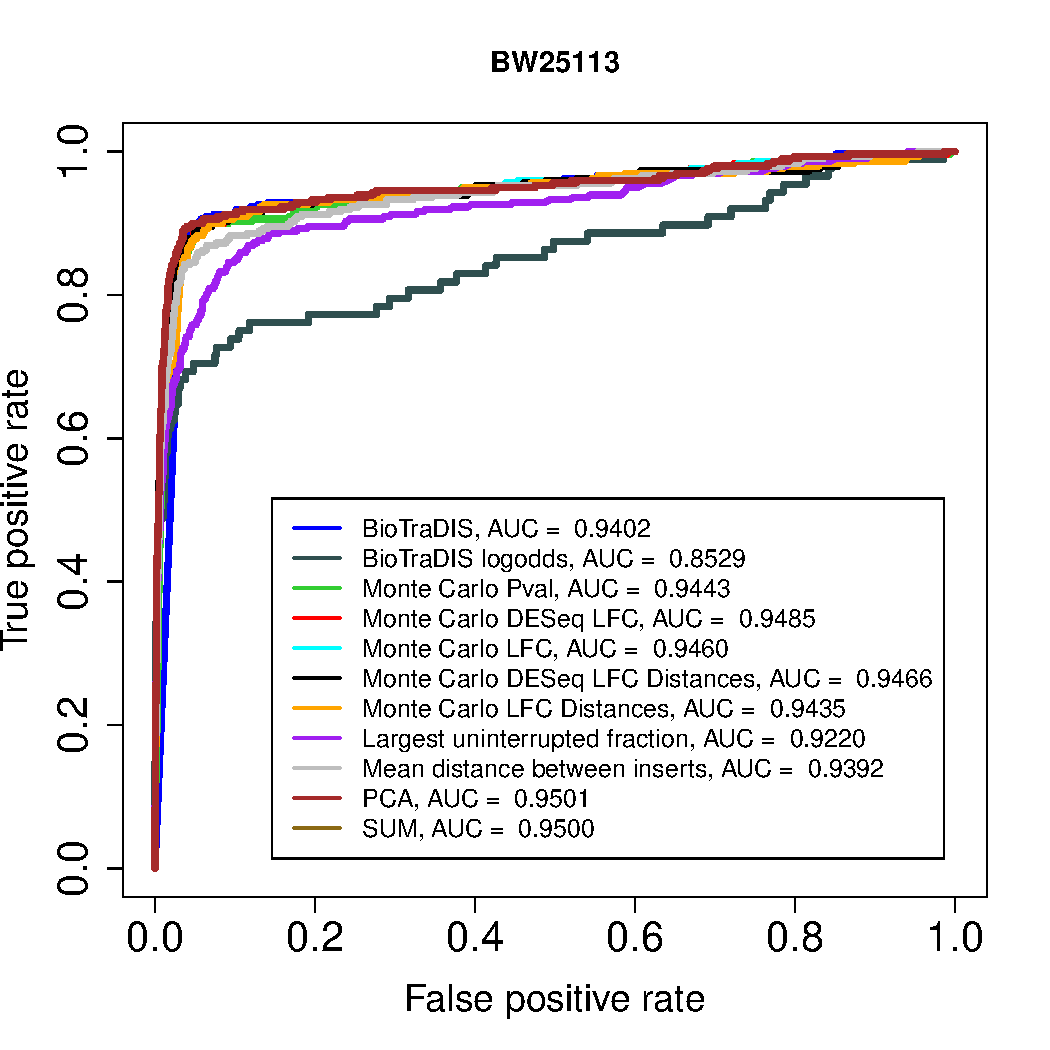
\includegraphics[page=1, scale=0.23]{essential-call-comparison-BW25113.pdf}&
%\includegraphics[page=1, scale=0.23]{essential-call-comparison-CS17.pdf}\\
%\includegraphics[page=1, scale=0.23]{essential-call-comparison-EC958.pdf}&
%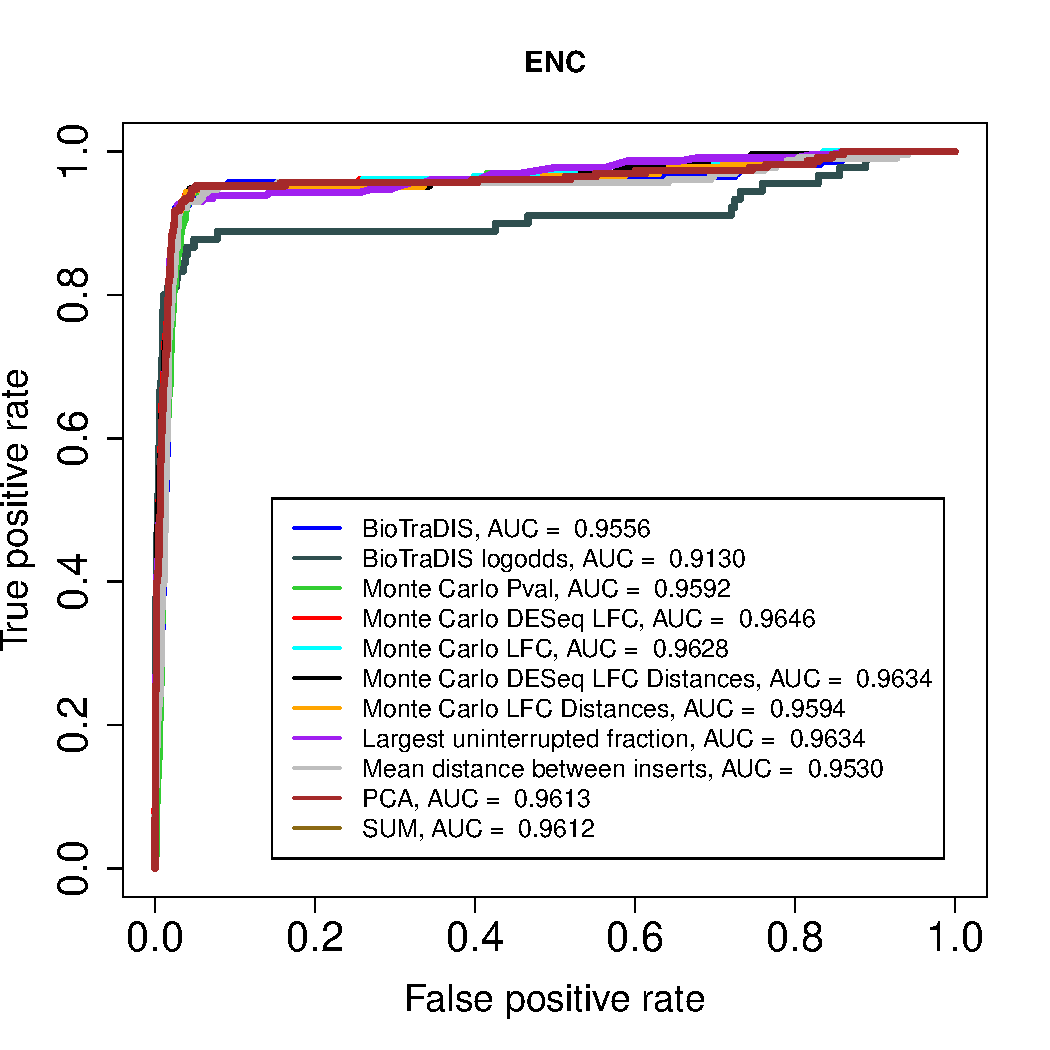
\includegraphics[page=1, scale=0.23]{essential-call-comparison-ENC.pdf}&
%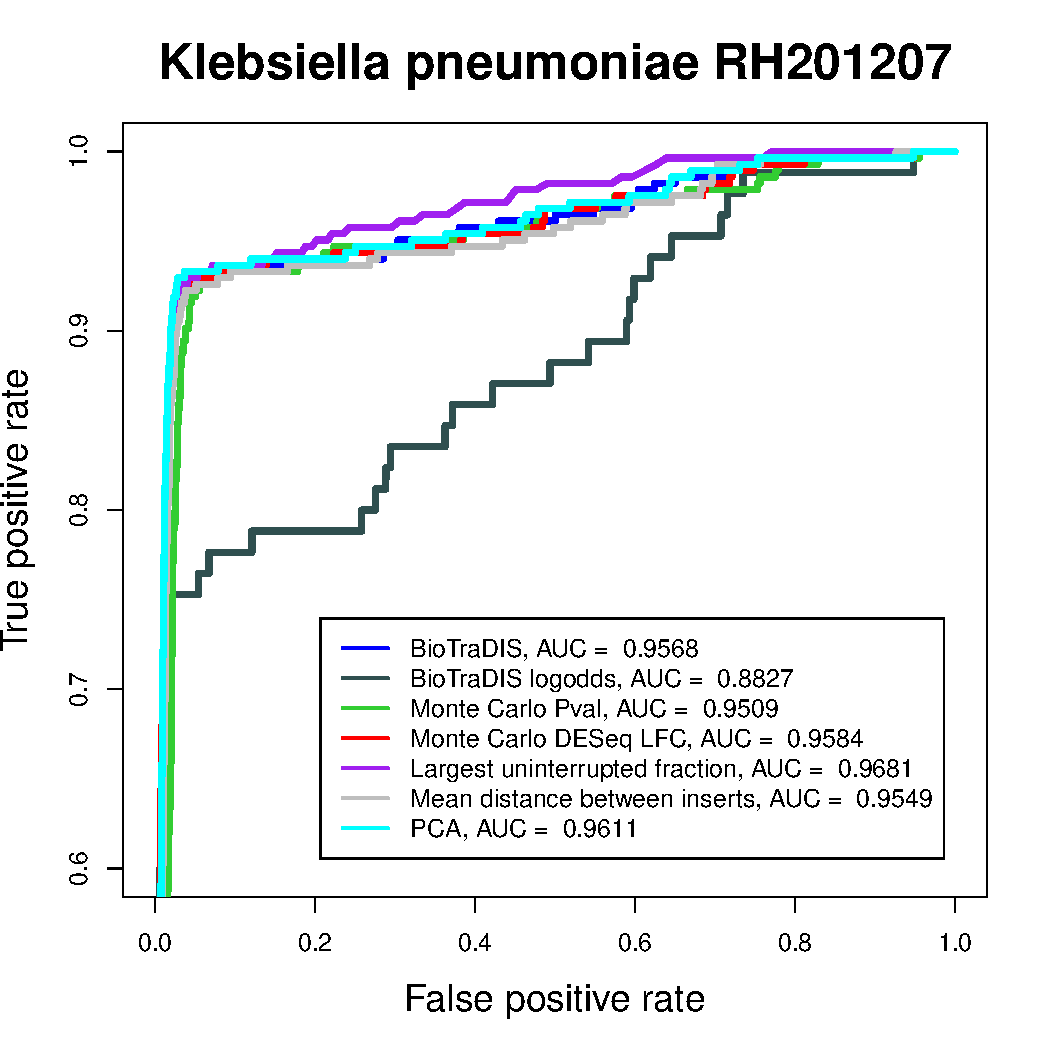
\includegraphics[page=1, scale=0.23]{essential-call-comparison-ERS227112.pdf}\\
%\includegraphics[page=1, scale=0.23]{essential-call-comparison-ETEC.pdf}&
%\includegraphics[page=1, scale=0.23]{essential-call-comparison-NCTC13441.pdf}&
%\includegraphics[page=1, scale=0.23]{essential-call-comparison-ROD.pdf}\\
%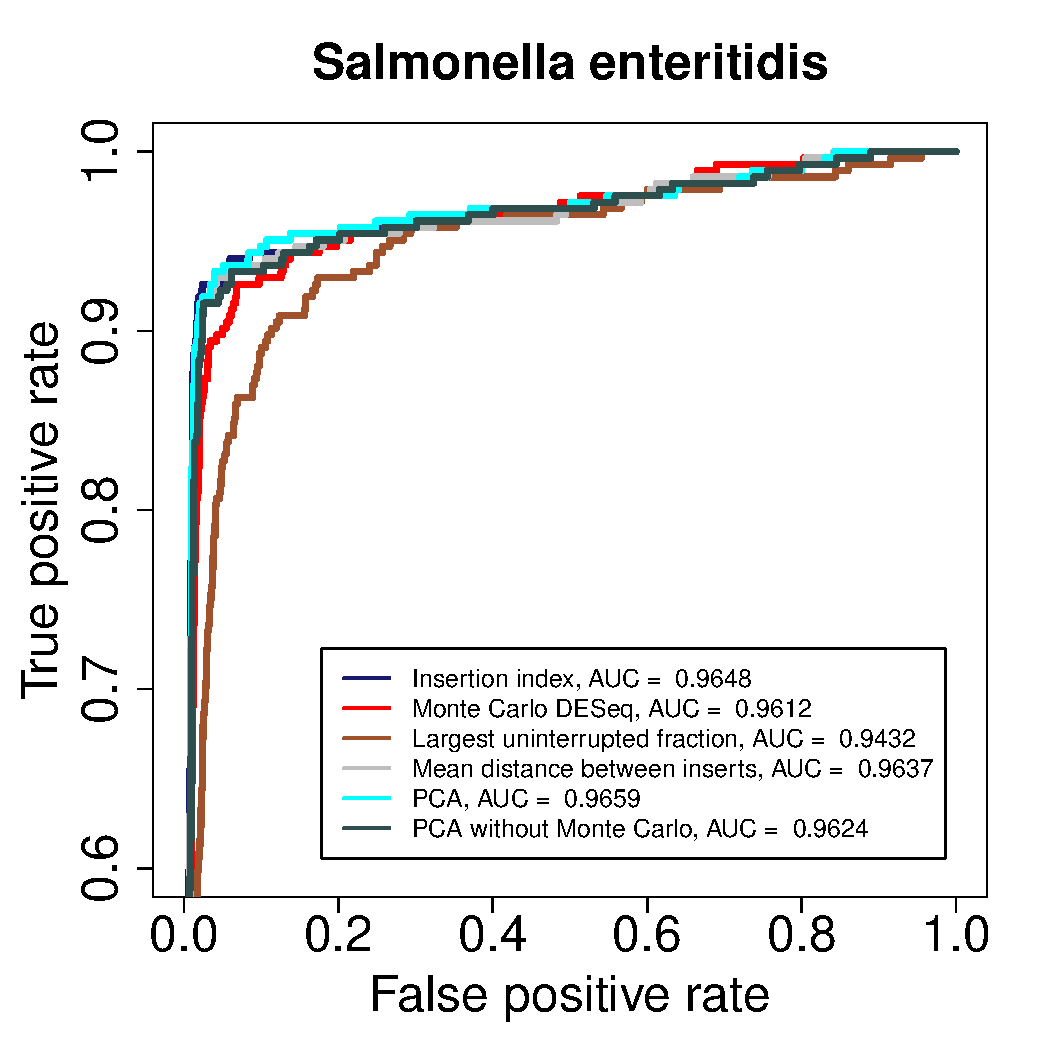
\includegraphics[page=1, scale=0.23]{essential-call-comparison-SEN.pdf}&
%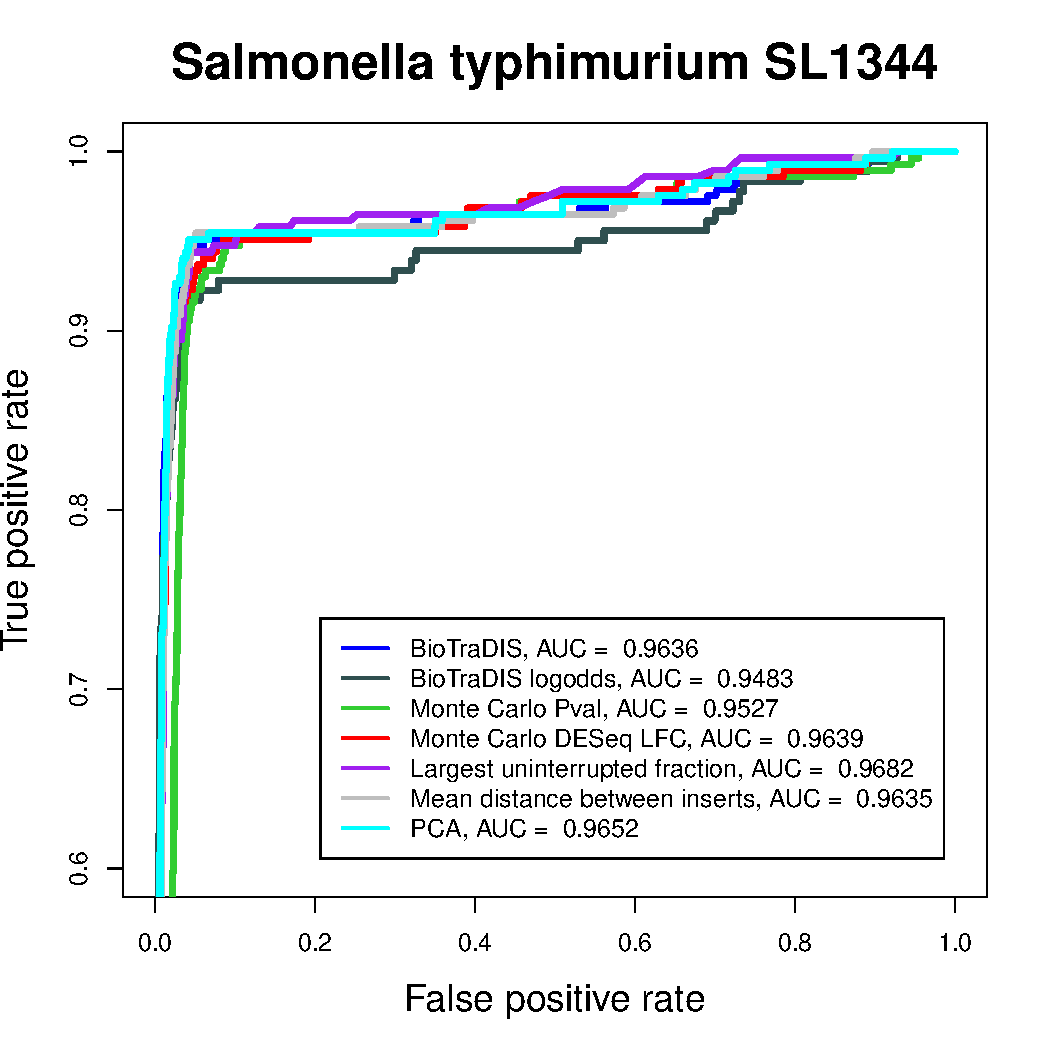
\includegraphics[page=1, scale=0.23]{essential-call-comparison-SL1344.pdf}&
%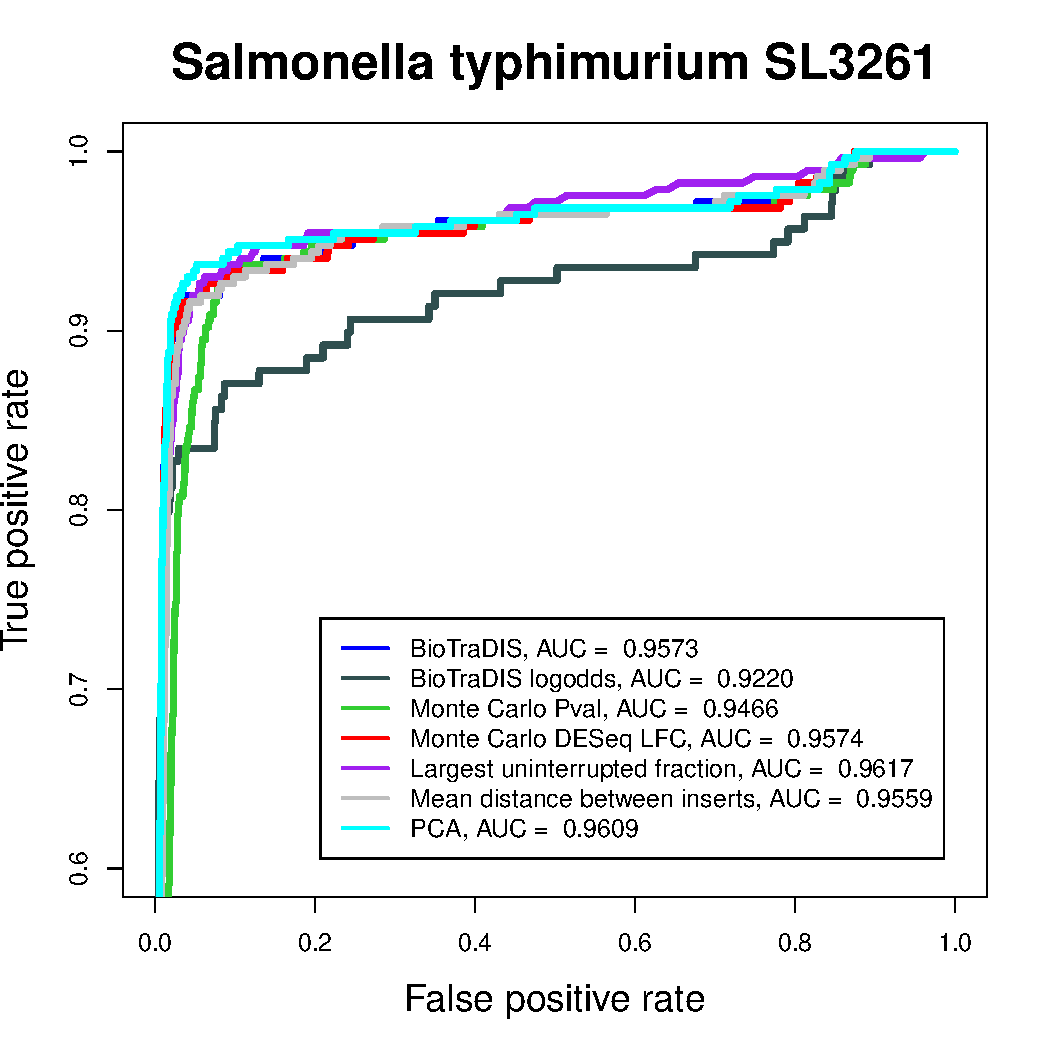
\includegraphics[page=1, scale=0.23]{essential-call-comparison-SL3261.pdf}\\
%\includegraphics[page=1, scale=0.23]{essential-call-comparison-STM.pdf}&
%\includegraphics[page=1, scale=0.23]{essential-call-comparison-STMMW.pdf}&
%\includegraphics[page=1, scale=0.23]{essential-call-comparison-t.pdf}\\
%\end{tabular}
%\caption{The plots show the accuracy of 7 different prediction methods for quantifying the essentiality of genes. The higher the area under the curve, the more accurate the method is.}
%\label{fig:benchmark}
%\end{figure*}

%\begin{figure*}
%\centering
%\begin{tabular}{c c c}
%\includegraphics[page=10, scale=0.22]{essential-call-comparison-BN373.pdf}&
%\includegraphics[page=10, scale=0.22]{essential-call-comparison-BW25113.pdf}&
%\includegraphics[page=10, scale=0.22]{essential-call-comparison-CS17.pdf}\\
%\includegraphics[page=10, scale=0.22]{essential-call-comparison-EC958.pdf}&
%\includegraphics[page=10, scale=0.22]{essential-call-comparison-ENC.pdf}&
%\includegraphics[page=10, scale=0.22]{essential-call-comparison-ERS227112.pdf}\\
%\includegraphics[page=10, scale=0.22]{essential-call-comparison-ETEC.pdf}&
%\includegraphics[page=10, scale=0.22]{essential-call-comparison-NCTC13441.pdf}&
%\includegraphics[page=10, scale=0.22]{essential-call-comparison-ROD.pdf}\\
%\includegraphics[page=10, scale=0.22]{essential-call-comparison-SEN.pdf}&
%\includegraphics[page=10, scale=0.22]{essential-call-comparison-SL1344.pdf}&
%\includegraphics[page=10, scale=0.22]{essential-call-comparison-SL3261.pdf}\\
%\includegraphics[page=10, scale=0.22]{essential-call-comparison-STM.pdf}&
%\includegraphics[page=10, scale=0.22]{essential-call-comparison-STMMW.pdf}&
%\includegraphics[page=10, scale=0.22]{essential-call-comparison-t.pdf}\\
%\end{tabular}
%\caption{The plots show the distribution of our new prediction method which is calculated by running PCA on insertion index, log fold change using sampling and DESeq, the average distance between insertion sites in a gene, and the length of the longest uninterrupted region and selecting first principal component. This method is called NPEQ.}
%\label{fig:pca}
%\end{figure*}
\subsection{TraDIS data is biased}
In Section~\ref{sec:essentiality-call} we proposed NPEQ method that quantifies the level of essentiality of a gene. However, if the transposon insertion is biased to specific regions in the genome, it can increase/decrease the values predicted by our method for genes and put them in a different level of essentiality. Different articles have reported biases in transposon insertion using Tn5 \cite{barquist_comparison_2013, green_insertion_2012, rubin_essential_2015, canals_high-throughput_2012, langridge_simultaneous_2009}. We performed a detailed study of these biases. The biases that we studied include: origin of replication bias, preferred insertion motif bias, and positional bias within genes.
\subsubsection{Distance from the origin of replication bias}
While a study has reported Tn5 insertion bias near the origin of replication \cite{barquist_comparison_2013}, another study has reported no bias \cite{rubin_essential_2015}. To study the bias towards the position of gene within genome, we plotted NPEQ for each gene versus the distance of the gene from the origin of replication normalised by the length of the genome in Fig.\@ \ref{fig:distance-bias}. The figure indicates that NPEQ increases when the genes are located further from the origin of replication. When the bacteria are under replication during the transposn insertion process, there are more copies of the genes close to the origin of replication than the genes further away due to the initiation of different replication forks. This results in more insertions in the genes near the origin of replication which can influence the accuracy of our predictions.
%One might argue that the bias that we have observed may have happened due to the abundance of essential genes near the origin of replication. Rocha and Eduardo \cite{rocha_replication-related_2004} have shown that unlike highly expressed genes, essential genes are not enriched near the origin of replication.

\begin{figure}
\captionsetup[subfigure]{justification=centering}
\begin{subfigure}{.49\textwidth}
  \centering
  \includegraphics[page=6, scale=0.25]{biases.pdf}
  \caption{}
  \label{fig:distance-bias}
\end{subfigure}
\begin{subfigure}{.49\textwidth}
  \centering
  \includegraphics[page=5, scale=0.25]{biases.pdf}
  \caption{}
  \label{fig:GC-bias}
\end{subfigure}
\begin{subfigure}{\textwidth}
  \centering
  \includegraphics[scale=0.6]{100logo-prob-edited.pdf}
  \caption{}
  \label{fig:logos}
\end{subfigure}
\begin{subfigure}{.49\textwidth}
  \centering
  \includegraphics[scale=0.25, page=2]{insertion-position-bias.pdf}
  \caption{}
  \label{fig:insertion-position-bias-ess}
\end{subfigure}
\begin{subfigure}{.49\textwidth}
  \centering
  \includegraphics[scale=0.25, page=4]{insertion-position-bias.pdf}
  \caption{}
  \label{fig:insertion-position-bias-ben}
\end{subfigure}
\caption{(a)The distance of the genes from DnaA gene normalised by the lengths of the genomes versus NPEQ. The distance from DnaA gene has been calculated in both directions and then the minimum value has been used for distance. The red curves show the loess curve when the smoothness parameter is $0.2$ and the green line shows no bias. (b) G-C content of genes against their NPEQ values. The red curves show the loess curve when the smoothness parameter is $0.2$ and the green line shows no bias. (c) Sequence logo plots generated using sequences from 10 nucleotides flanking the 100 top most frequent insertion sites from each genome. The height of each character shows the relative frequency of that character. (d) and (e) The plots show the average insertion index in percentiles of all essential genes (d) and beneficial losses (e). The genes are divided into 3 segments: 5\% of the genes on the $5^\prime$ end, 20\% of the genes on the $3^\prime$ end, and the rest in the middle. These are shown by khaki, slate gray, and violet red respectively.}
\label{fig:biases}
\end{figure}

%\begin{figure*}
%\centering
%\begin{tabular}{c c c}
%\includegraphics[page=2, scale=0.22]{biases.pdf}&
%\includegraphics[page=6, scale=0.22]{biases.pdf}&
%\includegraphics[page=10, scale=0.22]{biases.pdf}\\
%\includegraphics[page=14, scale=0.22]{biases.pdf}&
%\includegraphics[page=18, scale=0.22]{biases.pdf}&
%\includegraphics[page=22, scale=0.22]{biases.pdf}\\
%\includegraphics[page=26, scale=0.22]{biases.pdf}&
%\includegraphics[page=30, scale=0.22]{biases.pdf}&
%\includegraphics[page=34, scale=0.22]{biases.pdf}\\
%\includegraphics[page=38, scale=0.22]{biases.pdf}&
%\includegraphics[page=42, scale=0.22]{biases.pdf}&
%\includegraphics[page=46, scale=0.22]{biases.pdf}\\
%\includegraphics[page=50, scale=0.22]{biases.pdf}&
%\includegraphics[page=54, scale=0.22]{biases.pdf}&
%\includegraphics[page=58, scale=0.22]{biases.pdf}\\
%\end{tabular}
%\caption{The plots show the distance of the genes from DnaA gene normalised by the lengths of the genomes versus the insertion indices of the genes. The distance from DnaA gene has been calculated in both directions and then the minimum value has been used for distance. The red curves show the loess curve when the smoothness parameter is $0.2$.}
%\label{fig:distance-bias}
%\end{figure*}
\subsubsection{Preferred nucleotide composition bias}
Another concern while inferring essentiality from transposon insertion data is that transposon insertion is biased to certain compositions of nucleotides and high number of insertions in genes reflects the enrichment of the motifs that transposon insertion is biased towards, instead of their essentiality level. During Tn5 transposition, a sequence of 9 nucleotides is duplicated. Lodge et al. \cite{lodge_transposon_1988} showed that these duplicated regions have G-C pairs at two ends and replacing these G-C pairs with A-T pairs reduces the number of transposon insertions by more than fivefold. Goryshin et al. \cite{goryshin_tn5/is50_1998} reported the palindromic sequence A-GNTYWRANC-T as the consensus target site for Tn5 transposition where the 9 letters in middle show the consensus sequence in the duplicated region. %They have also showed that insertion sites are usually grouped together and have 5 base pairs distance from each other.
In some other research a similar consensus motif has been found for Tn5 \cite{canals_high-throughput_2012} which is CGCGCA-GTTYWRAAC-TGCGCG. Others \cite{green_insertion_2012,rubin_essential_2015} have not found such a sequence but shown that the duplicated regions are G-C rich. We used Weblogo~\cite{crooks_weblogo:_2004} to generate a logo from duplicated regions and 10 nucleotides flanking the 100 top most frequent insertion sites in each genome. The results in Figure \ref{fig:logos} show the consensus motif that we have found is very similar to \cite{green_insertion_2012} and the only difference is in positions 3 and 7 within the duplicated region.

%\begin{figure*}
%\includegraphics[scale=0.9]{100logo-prob-edited.pdf}
%\caption{Sequence logo plots generated using sequences from 10 nucleotides flanking the 100 top most frequent insertion sites from each genome. The height of each character shows the relative frequency of that character.}
%\label{fig:logos}
%\end{figure*}

The other possible source of bias is if transpositions are more inclined to G-C or A-T rich regions. Rubin et al. \cite{rubin_essential_2015} have reported that the number of Tn5 insertions rises with the increase of G-C content and Green et al. \cite{green_insertion_2012} have shown that the highest number of insertions occur in high G-C content regions. On the other hand, Langridge et al. \cite{langridge_simultaneous_2009} have seen an increase in the number of Tn5 insertions in 40\% G-C content. In Figure \ref{fig:GC-bias}, we plotted the G-C content of genes versus their NPEQ values. The red curves are loess curves with smoothness parameter 0.2 and the green line shows no bias. %In most cases (BW25113, EC958, ENC, ETEC, NCTC13441, ROD, SEN, STM, and t)
NPEQ decreases gradually (which means an increase in the number of insertions) as G-C content decreases and then somewhere between 40\% and 50\% G-C content, NPEQ starts to rise again in almost all genomes. %In three cases (SL1344, SL3261, and STMMW) NPEQ loess curve starts to fall off again at about 60\% G-C content which is probably due to a small number of genes with low NPEQ values in that region. The loess curve for BN373 is almost flat. In CS17, the loess curve goes down until it reaches the minimum value (at about 48\%) and then remains unchanged and in ERS227112, the NPEQ value is low at the beginning and then it increases at around 50\% G-C content.
In the region where most of the genes are packed, the loess curve is almost flat. On the left side of this flat region, there are genes with different G-C content which are enriched in mobile genetic elements. So, we expect to see more insertions (smaller NPEQ values) in this region. We have low NPEQ values between 40\% and 50\% G-C content which is expected. However, in most cases when we have less than 40\% G-C content, NPEQ value is high. A possible reason for this phenomena is the association of A-T rich sequences and histone-like nucleotide structuring (H-NS) proteins, which reduces the insertions in A-T rich regions. This has been shown for Tn10 transposon \cite{kimura_nucleoid_2016}, but not for Tn5 transposon, yet. Overall, the results are consistent with Langridge et al. \cite{langridge_simultaneous_2009}. The G-C content of the most of the genes with large NPEQ values is between 50\% and 60\% which is inconsistent with Green et al. \cite{green_insertion_2012} as this region contains most of the genes and is not considered as a high G-C content region but rather an average G-C content region. %Even though most of the regression lines are consistent with Rubin et al. results \cite{rubin_essential_2015}, the figures show that a linear regression cannot predict G-C bias as its slope changes dramatically in different datasets.

%\begin{figure*}
%\centering
%\begin{tabular}{c c c}
%\includegraphics[page=1, scale=0.23]{biases.pdf}&
%\includegraphics[page=5, scale=0.23]{biases.pdf}&
%\includegraphics[page=9, scale=0.23]{biases.pdf}\\
%\includegraphics[page=13, scale=0.23]{biases.pdf}&
%\includegraphics[page=17, scale=0.23]{biases.pdf}&
%\includegraphics[page=21, scale=0.23]{biases.pdf}\\
%\includegraphics[page=25, scale=0.23]{biases.pdf}&
%\includegraphics[page=29, scale=0.23]{biases.pdf}&
%\includegraphics[page=33, scale=0.23]{biases.pdf}\\
%\includegraphics[page=37, scale=0.23]{biases.pdf}&
%\includegraphics[page=41, scale=0.23]{biases.pdf}&
%\includegraphics[page=45, scale=0.23]{biases.pdf}\\
%\includegraphics[page=49, scale=0.23]{biases.pdf}&
%\includegraphics[page=53, scale=0.23]{biases.pdf}&
%\includegraphics[page=57, scale=0.23]{biases.pdf}\\
%\end{tabular}
%\caption{The plots show G-C content of genes against their NPEQ values. The red curves show the loess curve when the smoothness parameter is $0.2$ and the green line shows the linear regression line.}
%\label{fig:GC-bias}
%\end{figure*}

\subsubsection{Positional bias within genes}
Some research has indicated that himar1 transposons are more probable to get inserted into the two ends of a gene compared to the middle \cite{griffin_high-resolution_2011}. We have tested this hypothesis using our TraDIS data. We divided every gene into 100 fragments with equal lengths (percentiles) and calculated the mean insertion index for each percentile. Insertion index is calculated using $\frac{\frac{n_p}{l_p}}{\frac{n_g}{l_g}}$, where $n_p$ is the number of insertion sites in a specific percentile, $l_p$ is the length of that percentile, $n_g$ is the number of insertion sites in the whole genome and $l_g$ is genome length. Mean insertion index for each percentile is calculated by averaging over all insertion indices for that specific percentile of genes. We saw almost no bias towards any location when considering all genes together (Fig.\@ \ref{fig:insertion-position-bias} {\color{red}SUPPLEMENTARY}). We studied the bias in three different groups of genes: essential genes which have no or just a few insertions, non-essential genes which have an intermediate number of insertions, and beneficial losses which have a high number of insertions. The results imply that the number of insertions in the internal region of the essential genes is outnumbered by the number of insertions in the $5^\prime$ and $3^\prime$ ends (Fig.\@ \ref{fig:insertion-position-bias-ess}) while it is the opposite in beneficial losses (Fig.\@ \ref{fig:insertion-position-bias-ben}). High number of insertions at the $3^\prime$ end of essential genes implies that the functional domains are located before the insertions and the insertions are not interfering with them. On the other hand, high number of insertions at the $5^\prime$ end of the essential genes indicates there might be alternative start codons in the $5^\prime$ end or it might be because of annotation errors that have predicted the start codon in an incorrect place before the actual start codon.

%\begin{figure*}
%\begin{tabular}{c c}
%\includegraphics[scale=0.4, page=1]{insertion-position-bias.pdf}&
%\includegraphics[scale=0.4, page=2]{insertion-position-bias.pdf}\\
%\includegraphics[scale=0.4, page=3]{insertion-position-bias.pdf}&
%\includegraphics[scale=0.4, page=4]{insertion-position-bias.pdf}
%\end{tabular}
%\caption{The plots show the average insertion index in the percentiles of all genes (top left), essential genes (top right), non-essential genes (bottom left), and beneficial losses (bottom right). The genes are divided into 3 segments: 5\% of
%the genes on the 5' end, 20\% of the genes on the 3' end, and the rest in the middle. These are shown by khaki, slate gray, and violet red respectively.}
%\label{fig:insertion-position-bias}
%\end{figure*}
\subsection{Most essential genes are ubiquitously essential in Enterobacteriaceae}
Previous studies of gene essentiality in Enterobacteriaceae family have compared essential genes in different genomes in this family and studied the sets of core essential genes and accessory essential genes \cite{freed_combining_2016, canals_high-throughput_2012, barquist_comparison_2013}. Core essential genes are responsible for essential processes such as cell division, DNA replication, transcription and translation and some important pathways like peptidoglycan and fatty acid biosynthesis \cite{barquist_comparison_2013}. Accessory essential genes differ in genomes due to different reasons such as niche adaptation, functional redundancy and the existence of alternative pathways \cite{freed_combining_2016, canals_high-throughput_2012, barquist_comparison_2013, bergmiller_patterns_2012}. Another group of accessory essential genes are phage repressors \cite{barquist_comparison_2013}. Even though these genes are not essential for the growth of a cell, once phages are introduced to a cell, they become essential as long as the phage remains in the cell.

In this study, we have compared the genes in 16 bacteria from Enterobacteriaceae family. For this we needed to study core and accessory sets of genes. Moreover, in the presence of two redundant variations of one gene, if we knock out one copy using TraDIS, the other copy compensates and the organism can still survive \cite{bergmiller_patterns_2012,dean_pervasive_2008}. This leads to a different essentiality inference using TraDIS. Therefore, in addition to core and accessory genes, we have studied duplicate genes. To study whether each gene in the 16 organisms is core, we used Jackhmmer from HMMER package~\cite{eddy_accelerated_2011} to iteratively search for homologous proteins in our dataset and cluster them. We divided the clusters of homologous genes into three groups based on their conservation. Genus specific class contains genes that are present only in one genus, the genes in single copy class are present in more than one genus and more than 70\% of them are not duplicated (core genes), and  the genes in multi-copy class are present in more than one genus and more than 30\% of them are duplicated (duplicate genes).

We also evaluated the essentiality of genes and divided the genes into different levels of essentiality using NPEQ values. If NPEQ is less than -1.644854, it means that the gene has tolerated many insertions, so it is beneficial for the organism to lose this gene in the rich medium that we used. However, if NPEQ is greater than 1.644854, the gene can tolerate very few or no insertions indicating that the gene is essential for cell viability in our test medium. Any other NPEQ value shows an intermediate number of insertions in genes meaning that it is not beneficial for the organism to lose these genes, but they are not essential, too. We have called this group of genes non-essential.

The results for comparing three levels of essentiality and three classes of conservation are depicted in Fig.\@ \ref{fig:iidist}. The high number of single copy clusters in essential level, indicates that there is a set of essential genes in Enterobacteriaceae that are conserved and inclined to keep their essentiality. However, there are also many essential genus specific genes. The figure also shows that beneficial losses are over represented in genus specific class. Therefore, beneficial losses are mostly recent genes that the organism tends to lose in the long run. Besides, most of the multi-copy clusters are non-essential and there are only a few multi-copy clusters that are essential. This can be explained by the redundancy that duplicate genes can keep even after $\sim100$ million years \cite{dean_pervasive_2008}. 

\begin{figure}
\captionsetup[subfigure]{justification=centering}
\begin{subfigure}{.5\textwidth}
  \centering
  \includegraphics[scale=0.4]{cluster-essentiality.pdf}
  \caption{}
  \label{fig:iidist}
\end{subfigure}%
\begin{subfigure}{.5\textwidth}
  \centering
  \includegraphics[scale=0.4]{essential-pathways.pdf}
  \caption{}
  \label{fig:essentiality-pathway-ess}
\end{subfigure}
\begin{subfigure}{.5\textwidth}
  \centering
  \includegraphics[scale=0.4]{non-essential-pathways.pdf}
  \caption{}
  \label{fig:essentiality-pathway-nes}
\end{subfigure}
\begin{subfigure}{.5\textwidth}
  \centering
  \includegraphics[scale=0.4]{beneficialloss-pval.pdf}
  \caption{}
  \label{fig:essentiality-pathway-ben}
\end{subfigure}
\caption{(a) The genes have been clustered into homologous groups using Jackhmmer and divided into 3 groups: genus specific, single copy, and multi-copy genes. Then, the essentiality of the clusters has been defined using the insertion indices of the genes in the clusters. The figure shows that most of the essential genes are in single copy group, while most of the beneficial losses are genus-specific. (b) and (c) KEGG Pathways enriched in essential genes (b) and non-essential genes (c). (d) The words enriched in the description of beneficial losses in their embl files compared to other genes. The red line shows P-value = 0.05. The P-values are calculated using hypergeometric test and then corrected using Benjamini-Hochberg-Yekutieli procedure.}
\label{fig:gene-classes}
\end{figure}

%\begin{figure}
%\centering
%\includegraphics[scale=0.5]{cluster-essentiality.pdf}
%\caption{The genes have been clustered into homologous groups using Jackhmmer and divided into 3 groups: genus specific, single copy, and multi-copy genes. Then, the essentiality of the clusters has been defined using the insertion indices of the genes in the clusters. The figure shows that most of the essential genes are in single copy group, while most of the beneficial losses are genus-specific.}
%\label{fig:iidist}
%\end{figure}

To study which functions are enriched in each class of essentiality, we used KEGG pathway enrichment analysis \cite{kanehisa_kegg:_2000} and compared the genes in each class with the databases that were available for the genomes in this study. The results show that essential genes are enriched in pathways related to genetic information processing such as replication (DNA replication, homologous recombination and mismatch repair), transcription (RNA polymerase), translation (ribosome), and protein export. These are the essential functions that every cell needs for its viability. Other enriched pathways are mostly metabolism related. These include fatty acid biosynthesis that produces cell membrane, peptidoglycan and lipopolysaccharide biosynthesis that are essential components of cell wall, terpenoid backbone biosynthesis which feeds peptidoglycan biosynthesis, nucleotide and amino acid metabolism, and the metabolism of important cofactors and vitamins like riboflavin, biotin,porphyrin and chlorophyll (Figure~\ref{fig:essentiality-pathway-ess}).
{\color{red} CAN WE HAVE SOMETHING LIKE THIS? http://www.nature.com/articles/srep00125}

Non-essential genes are mostly involved in carbohydrate, energy, and lipid metabolism, membrane transport, cell motility and cellular community. Even though these functions are important, they are not essential in a rich medium in lab.

As most of beneficial losses do not have homologs in other genomes, most of them are not studied and therefore there is no KEGG pathway for them. Because of this reason, we studied the description of these genes in their embl files and found the words that were enriched. These are shown in Figure~\ref{fig:essentiality-pathway-ben}. The results show that most of beneficial losses are mobile genetic elements like transposases and insertion elements which are not essential in their host genomes, genes that are not essential in a rich medium like stress protein and acid-resistance protein, and hypothetical proteins.
%\begin{figure*}
%\centering
%\begin{tabular}{c c}
%\includegraphics[scale=0.4]{essential-pathways.pdf}&
%\includegraphics[scale=0.4]{non-essential-pathways.pdf}\\
%\includegraphics[scale=0.4]{beneficialloss-pathways.pdf}&
%\includegraphics[scale=0.4]{beneficialloss-pval.pdf}
%\end{tabular}
%\caption{Pathway enrichment analysis for beneficial losses, essential genes, and non-essential genes compared to other genes. The red line shows P-value = 0.05. The P-values are calculated using hypergeometric test and then corrected using Benjamini-Hochberg-Yekutieli procedure.}
%\label{fig:essentiality-pathway}
%\end{figure*}

%\subsection{Phylogenetic analysis of gene essentiality identifies that essential genes are more likely to be conserved}

%When a mutation is introduced to a gene, the fixation rate depends on how tolerable this mutation is \cite{wilson_biochemical_1977}. As mutations in essential genes are less likely to be tolerable, less mutations should be fixed in these genes, and therefore essential genes should evolve more slowly than non-essential genes. This is known as knockout rate hypothesis \cite{krylov_gene_2003}. Different studies have verified this hypothesis in prokaryotes \cite{jordan_essential_2002, gerdes_experimental_2003, rocha_analysis_2004, silander_constancy_2009}.

We have shown that many of the essential genes are conserved. But are essential genes more likely to be conserved? To answer this question, we have compared the number of ancestrally essential genes and ancestrally present genes in the phylogenetic tree as we go up to the root. We have used Fitch's algorithm \cite{fitch_toward_1971} with a binary alphabet on both essentiality (0 for non-essential and 1 for essential) and conservation (1 for the presence and 0 for the absence of genes) to define if a gene is ancestral essentially or present at each level in the phylogenetic tree. If we get 1 at the top of the tree while studying essentiality of a gene using Fitch's algorithm, it means that the gene is ancestrally essential and otherwise, the gene is ancestrally non-essential. The same applies to the study of ancestrally present genes. The phylogenetic tree has been annotated with the number of ancestrally essential genes (red) and the number of ancestral genes (blue) at each level in Figure~\ref{fig:tree}. We then plotted the ratios at each level in the phylogenetic tree in Figure~\ref{fig:fitch} and connected the medians in each level. The connecting line shows that the ratio between ancestrally essential genes and ancestral genes rises as we go higher in the phylogenetic tree which means essential genes are more likely to be conserved in genomes compared to non-essential genes.

\begin{figure}
\captionsetup[subfigure]{justification=centering}
\begin{subfigure}{.6\textwidth}
  \centering
  \includegraphics[scale=0.12]{phylosift-aa-raxmlbootstrap-annotated.pdf}
  \caption{}
  \label{fig:tree}
\end{subfigure}
\begin{subfigure}{.4\textwidth}
  \centering
  \includegraphics[scale=0.4]{fitch.pdf}
  \caption{}
  \label{fig:fitch}
\end{subfigure}
\caption{(a) The species tree for all genomes in this study. Numbers in red show the number of ancestrally essential genes at each level and numbers in blue show the number of ancestral genes at each level. (b) The ratio between ancestrally essential genes and ancestral genes at each level in the species tree. The dots in the strain level show the ratios for all 16 bacteria; the dots in the species level show the ratios for Enterobacter, Klebsiella, Citrobacter, Salmonella, and Escherichia; the subfam. level shows the ratios for the common ancestor of Enterobacter and klebsiella, the common ancestor of Citrobacter and Salmonella, and the common ancestor of Citrobacter, Salmonella, and Escherichia; and finally the dot in the family level shows the ratio for the root. The line connects the medians in each level.}
\label{fig:essentiality-phylogeny}
\end{figure}

We have studied the essentiality status of genes involved in important biological processes in Table~\ref{tab:biological-processes}. These processes include cell division, DNA replication, transcription, translation, and important metabolic pathways such as peptidoglycan and fatty acid biosynthesis. If a gene was not ancestrally essential using Fitch's algorithm, we looked at its essentiality in every genome: if it was essential in some of the genomes we classified it as ambiguous and if it was not essential in any genome we classified it as ancestrally non-essential.
%FtsA and zipA genes are essential for cell division. FtsA is essential in all the genomes in our study, however zipA is essential everywhere except for Salmonella typhimurium A130 in which this gene is near essential. We investigated if this gene has a homolog in Salmonella typhimurium A130 and found no homologs. It has been shown that 21 mutations in ftsA gene can make it independent of zipA gene so that the zipA gene is no longer essential \cite{geissler_gain--function_2003, pichoff_ftsa_2012}. However, ftsA gene does not have any of these mutations in Salmonella typhimurium A130, so there might be another factor that is causing zipA not to be essential. \textcolor{red}{ADD MORE EXAMPLES HERE}

\begin{landscape}
\begin{table}
\small
\caption{The essentiality status of genes involved in important biological processes}
\label{tab:biological-processes}
\begin{tabular}[t]{l l l l l}
\hline
\textbf{Biological process} & \textbf{Subprocess} & \textbf{Ancestrally essential} & \textbf{Ambiguous} & \textbf{Ancestrally non-essential}\\
\hline
Cell Division & & \begin{tabular}[t]{@{}l@{}}ftsAHLQWYZ, minE,\\ mukB, zipA \end{tabular}& ftsKNX, minD & \begin{tabular}[t]{@{}l@{}}CedA, ftsJ, minC,\\ sdiA, sulA\end{tabular}\\
DNA replication & Polymerases I, II, III & dnaENQX, holABD, polA & holC & holE, polB\\	
& Supercoiling & gyrAB, parCE & & \\
& Primosome-associated & dnaBCGT, priA, ssb & priB, rep & priC\\
Transcription & RNA polymerase & rpoABC &  & \\
& \begin{tabular}[t]{@{}l@{}}Sigma, elongation, anti- \\ and termination factors\end{tabular} & nusABG, rho, rpoDH & rpoEN & rpoS\\	
Translation & tRNA-synthetases & \begin{tabular}[t]{@{}l@{}}alaS, argS, asnS, aspS, cysS, \\ glnS, gltX, glyQS, hisS, ileS, \\ leuS, lysS, metG, pheST, \\ proS, serS, thrS, tyrS, valS \end{tabular} & trpS	 & \\	
& Ribosome components & \begin{tabular}[t]{@{}l@{}}rplBCDEFJKLMNOPQRSTUV,\\ rplWXY, rpmABCD,\\ rpsABCDEFGHJKLMNPQRSTU\end{tabular} & \begin{tabular}[t]{@{}l@{}}rplA, rpmEGHI,\\ rpsIO\end{tabular} & rplI, rpmF\\
& \begin{tabular}[t]{@{}l@{}}Initiation, elongation \\ and peptide chain \\ release factors\end{tabular} & fusA, infABC, prfAB, tsf & efp & prfC, selB, tufAB \\
Biosynthetic pathways & & & & \\
Peptidoglycan & & MraY, murABCDEFGI & & ddlAB\\	
Fatty acids & & accABCD, fabABDGHIZ & & \\
\hline
\end{tabular}
\end{table}
\end{landscape}

%So far we have shown that essential genes are less likely to be lost during evolution. The other question is if essential genes tend to keep their essentiality in different genomes. Bergmiller et al. \cite{bergmiller_patterns_2012} have shown that only essential genes whose functions cannot be taken over by other genes keep their essentiality and others are possible to be lost or non-essential in other genomes. The genes that can replace other genes are not necessarily homologous to them, but they have similar functions.
Genes that are essential in one organism can be non-essential or absent in other organisms. Bergmiller et al. \cite{bergmiller_patterns_2012} have studied 26 genes that are essential in E. \textit{coli}. Some of these genes are essential in other bacteria and some are non-essential or not present in other bacteria. In 10 cases, they were able to find genes that compensate for these essential genes if they are overexpressed and called these genes high copy suppressors. High copy suppressors are not necessarily similar to their counterpart essential genes in structure or sequence, but they have similar functions. They have shown that genes that are not present or essential everywhere are more likely to be compensated for by overexpression of another gene. The other reason for genes to lose their essentiality in some strains is changes in their physiology or environment \cite{barquist_comparison_2013}.

We have compared the number of genes that are shared between our bacterial genomes (\ref{fig:upsetr-conservation}) and the number of genes essential in them (\ref{fig:upsetr-essentiality}) and used UpSetR package \cite{conway_upsetr:_2016} to visualise the results in Fig.\@ \ref{fig:upsetr}. As shown in the figures, among 2162 genes that are shared between all the bacteria under study, only 135 are essential everywhere and many of the essential genes are not conserved or essential everywhere probably because of their compensability, physiological, or environmental changes. %We looked at subsets of the genes that were shared in every combination of our bacterial strains to see whether they show a trend similar to the phylogenetic tree. The results propose that although conservation of genes follows a tree-like trend, the essentiality does not show such a trend. The reason is that many of the essential genes that are not shared in all genomes are probably compensable by other genes and so the essentiality does not look tree-like.



\begin{figure}
\captionsetup[subfigure]{justification=centering}
\begin{subfigure}{.5\textwidth}
  \centering
  \includegraphics[scale=0.45,page=2]{upsetr.pdf}
  \caption{}
  \label{fig:upsetr-conservation}
\end{subfigure}
\begin{subfigure}{.5\textwidth}
  \centering
  \includegraphics[scale=0.45,page=3]{upsetr.pdf}
  \caption{}
  \label{fig:upsetr-essentiality}
\end{subfigure}
\caption{(a) The number of genes and (b) essential genes shared between different groups of bacteria. The bars show the number of genes and the filled circles show which bacteria are sharing those genes.}
\label{fig:upsetr}
\end{figure}

%\section{Discussion}
\section{Materials and Methods}
%\subsection{Transposon insertion}
%\section{Results and discussion}
%Throughout time, species can gain or lose genes. We investigated if these gene gain and losses are related to the essentiality of the genes. In this section, we have first described the biases that can affect our study, and then evaluated the essentiality of genes and their conservation and the relationship between these two.
%
%
%%\subsection{Length bias}
%%Short genes are less probable to be hit by transposons and so the genes that are very short might have no insertions. As a result, normalising the number of insertions by the length of the genes does not affect the essentiality level of these genes. 
%%In Fig.\@ \ref{fig:length-bias} we have studied if the length of genes can influence their essentiality and we have found no correlation between length and insertion index in short genes. It seems that the insertion density in our experiment is high enough to make it possible for every gene to be hit by transposons.
%%\begin{figure*}
%%\centering
%%\includegraphics[page=42, scale=0.3]{biases.pdf}
%%\caption{The plot shows the lengths of the genes against their insertion indices. The red line shows the loess curve when the smoothness parameter is $0.2$.}
%%\label{fig:length-bias}
%%\end{figure*}
%
%
%\subsubsection{Preferred insertion motif bias}

%
%\begin{itemize}
%\item model H-NS binding sites? CGWTWHWww Lang et al (2007)
%\item seems unlikely -- show bulk of genes are around 50\% G+C (add box-whisker plots to scatter diagrams?)
%\item check Freed, Silander paper -- the missing piece of genome, was this low G+C? It is not mentioned in the paper.
%\end{itemize}
%
%\begin{figure*}
%\includegraphics[scale=0.55]{lowgc-pval.pdf}
%\caption{Word enrichment analysis for low G-C genes compared to genes with interquartile G-C level. The red line shows P-value = 0.05. The P-values have been calculated using Fisher's exact test and corrected using Benjamini-Hochberg-Yekutieli.}
%\label{fig:gc-pval}
%\end{figure*}
%

%\subsection{Essentiality and conservation}
%Essential genes are needed for the growth of organisms. Because of that, one might think that essential genes should not be lost in a short period of time throughout evolution, unless they are no longer needed in new organisms or they are replaced by new pathways. Therefore, it is expected that most of the essential genes are conserved in different organisms from the same family. We have tested this idea by comparing the essentiality and conservation of genes in Enterobacteriaceae family.
%
%
%\subsubsection{Gene classes}
%%We needed to cluster sets of orthologous genes in our strains to study the conservation of essentiality. Plenty of methods are proposed for this purpose. Altenhoff et al.\@ have compared 15 of these methods \cite{altenhoff_standardized_2016} and shown that Hieranoid \cite{schreiber_hieranoid:_2013} is among three methods that keep a balance between precision and recall. We have used Hieranoid to cluster the sets of orthologous genes. In addition, we intended to study the essentiality of genes in paralogous genes. For this, we have developed a program that clusters all homologous genes using Jackhmmer from HMMER3 package \cite{mistry_challenges_2013}.
%In order to study the relationship between essentiality and conservation, we needed to evaluate the essentiality and conservation of genes. For this, we divided the genes into different levels of essentiality (essential genes, ambiguous, non-essential genes, beneficial losses). We first normalised the biases that exist in the data using the method explained in Section~\ref{sec:biascorrection} and then defined the essentiality level of genes using the method explained in Section~\ref{sec:essentiality}. Moreover, we grouped the genes into different classes of conservation (genus specific, single copy, multi-copy) using the method explaind in Section~\ref{sec:conservationclasses}.
%
%The results for comparing four levels of essentiality and three classes of conservation are depicted in Fig.\@ \ref{fig:iidist}. The high number of single copy genes in essential level, indicates that there is a set of essential genes in Enterobacteriaceae that are conserved and inclined to keep their essentiality. However, the relatively high number of essential genes in genus specific class implies that each genus has a set of essential genes that makes it distinct. The figure also shows that beneficial losses are over represented in genus specific class. Therefore, beneficial losses are mostly recent genes that the organism tends to lose in the long run. Besides, most of the multi-copy clusters are non-essential and there are only a few multi-copy clusters that are essential. This can be explained by the redundancy that genes can keep even after $\sim100$ million years \cite{dean_pervasive_2008}. In the presence of two redundant variations of one gene, if we knock out one copy by transposon mutagenesis, the other copy compensates and the organism can still survive.
%
%\begin{figure}
%\centering
%\includegraphics[scale=0.5]{cluster-essentiality.pdf}
%\caption{The genes have been clustered into orthologous groups using Hieranoid and paralogous groups using Jackhmmer and divided into 3 groups: genus specific, single copy, and multi-copy genes. Then, the essentiality of the clusters has been defined using the insertion indices of the genes in the clusters. The figure shows that most of the essential genes are in single copy group, while most of the beneficial losses are genus-specific.}
%\label{fig:iidist}
%\end{figure}
%
%To study which functions are enriched in each class of essentiality, we used the word enrichment method explained in Section~\ref{sec:enrichment}. Fig.\@ \ref{fig:essentiality-pval} shows the top 20 enriched words for each essentiality class. The results show an enrichment of the genes related to replication, transcription, translation, division, and rod shape determining proteins in essential class. The non-essential genes are mostly membrane associated proteins, flagellar proteins, ATPase, and DNA repair proteins. Beneficial losses are enriched in transposase enzymes, putative and hypothetical proteins, and mobile elements. Beneficial losses also contain many fimbrial proteins which probably has occurred because these proteins are not needed in a rich lab medium \textcolor{red}{\{TRUE?\}}.
%%We have done a word enrichment analysis on the description of the beneficial losses in Fig.\@ \ref{fig:essentiality-pval}. It shows that most of the beneficial losses are mobile elements. Most of these mobile elements are not included in KEGG database.
%
%We also conducted a pathway enrichment analysis for these three groups which is explained in Section~\ref{sec:enrichment}. The results (Fig.\@ \ref{fig:essentiality-pathway}) suggest similar results to the enrichment analysis that we had done on the description of the genes. However, as mobile genetic elements are not stored in KEGG database \cite{kanehisa_kegg:_2000}, the pathway enrichment analysis does not show the enrichment of mobile genetic elements in beneficial-losses.
%
%\begin{figure*}
%\centering
%\begin{tabular}{c c}
%\includegraphics[scale=0.4]{essential-pval.pdf}&
%\includegraphics[scale=0.4]{non-essential-pval.pdf}\\
%\includegraphics[scale=0.4]{beneficialloss-pval.pdf}&
%\end{tabular}
%\caption{Word enrichment analysis for essential genes, non-essential genes, and beneficial losses compared to other genes. The red line shows P-value = 0.05. The P-values have been calculated using Fisher's exact test and then corrected using Benjamini-Hochberg-Yekutieli procedure.}
%\label{fig:essentiality-pval}
%\end{figure*}
%
%\begin{figure*}
%\centering
%\begin{tabular}{c c}
%\includegraphics[scale=0.4]{essential-pathways.pdf}&
%\includegraphics[scale=0.4]{non-essential-pathways.pdf}\\
%\includegraphics[scale=0.4]{beneficialloss-pathways.pdf}&
%\end{tabular}
%\caption{Pathway enrichment analysis for beneficial losses, essential genes, and non-essential genes compared to other genes. The red line shows P-value = 0.05. The P-values are calculated using hypergeometric test and then corrected using Benjamini-Hochberg-Yekutieli procedure.}
%\label{fig:essentiality-pathway}
%\end{figure*}
%
%\subsubsection{The evolution of essentiality}
%%In order to test if the essentiality of genes follows a tree-like trend we have gathered all the genes that are copied once per genome and made a matrix with rows showing genomes and columns showing genes. If a gene is essential in a genome, its corresponding cell in the matrix has value 1 and 0 otherwise. Then we have used the Bray-Curtis distance to generate a distance matrix for the species under study. Finally, a tree has been generated using PHYLIP Neighbor. The resulting tree is not similar to the species tree.
%%
%%\begin{figure}
%%\centering
%%\includegraphics[scale=0.2]{neighbor-joining-essentiality-tree.pdf}
%%\caption{The tree is generated from all the genes that are copied only once per genome. We have made a binary matrix from the essentiality of these genes. Then, we have generated a distance matrix from these values using Bray-Curtis distance and plotted a phylogenetic tree using PHYLIP Neighbor which uses a neighbour joining method.}
%%\label{fig:neighborjoining}
%%\end{figure}
%
%In this section, we compared the number of genes that were essential and conserved at each level of the phylogenetic tree. We were interested to see if the trend of the essentiality variation between different organisms is in agreement with the phylogenetic tree. In other words, we have tested if organisms close together have more essential genes in common than organisms that have separated earlier in the phylogenetic tree.
%
%We needed to cluster sets of orthologous genes in the bacteria that we were studying. Homologous clusters introduced in ~\ref{sec:conservationclasses} were not useful for this purpose as sets of paralogous genes with different essentiality levels can make essentiality inference ambiguous. Plenty of methods are proposed for this purpose. Altenhoff et al.\@ have compared 15 of these methods \cite{altenhoff_standardized_2016} and shown that Hieranoid \cite{schreiber_hieranoid:_2013} is among three methods that keep a balance between precision and recall. We used Hieranoid for clustering orthologous genes. Hieranoid need a species tree for clustering genes. We used the method explained in Section~\ref{sec:phylogenetic} to generate this tree.
%
%In order to test if the essentiality of genes follows a tree-like trend, we compared the number of genes that were conserved in different bacteria in our study and the number of genes that were essential in these bacteria. The genes that are conserved in all bacteria being studied are called core genes and the genes that are conserved and essential are called core essential genes. We counted the number of genes that were core between every combination of bacteria, and the number of core essential genes between those combinations. We used UpSetR package \cite{conway_upsetr:_2016} in R to visualise the results in Fig.\@ \ref{fig:upsetr}. As shown in the figures, among 1908 genes that are core between all the bacteria under study, only 184 are core essential. We looked at subsets of the genes that were core essential (core) in every combination of our bacterial strains to see whether they were phylogenetically informative or not. A phylogenetically informative subset is a subset that is core essential (core) in two or more bacteria but not in all bacteria. We have marked the phylogenetically informative sets of genes with ticks and the uninformative ones with crosses. The results propose that although conservation of genes follows a tree-like trend with many phylogenetically informative sets of genes with high cardinality, the essentiality does not show a tree-like signal and most of the large sets of core essential genes belong to only one bacteria. We believe this is due to the small number of essential genes. Each bacterium has about 300 to 500 essential genes among which 184 is core essential between all bacteria. A portion of the remaining essential genes are specific to each bacterium and many are shared between all bacteria except one. The number of remaining essential genes is so low that causes the essentiality trend not to be tree-like. Furthermore, some of the predicted essential genes might be artefacts of transposon mutagenesis method.
%
%\begin{figure*}
%\centering
%\includegraphics[scale=0.6, page=2]{upsetr-maximiseMCC.pdf}\\
%\includegraphics[scale=0.6, page=3]{upsetr-maximiseMCC.pdf}
%\caption{The first figure shows the number of core genes between each group of species and the second figure shows the number of core essential genes. The bars show the number of genes that are core between the strains marked with black circles. The tick marks show phylogenetically informative columns and the cross marks show non-informative columns.}
%\label{fig:upsetr}
%\end{figure*}
%
%To further study the trend of essentiality changes, we looked at different levels in the species tree and calculated the ratio of the number of core essential genes to the number of core genes in each level. We used three different methods for inferring core genes and core essential genes. These methods are explained in Section~\ref{sec:core}. The numbers predicted using these three methods are shown in Fig.\@ \ref{fig:annotated-speciestree}. As this figure shows, the ratio between core essential and core genes is almost constant using the intersection and dollo method; however, this ratio increases as we go higher in the tree using the ancestral insertion index method.
%
%%\begin{figure}
%%\centering
%%\includegraphics[scale=0.2]{phylosift-aa-raxmlbootstrap-annotated.pdf}
%%\caption{The tree shows the species tree in Fig.\@\ref{fig:species-tree} annotated by the number of core essential genes and core genes at each node. We used three methods to define core essential genes and core genes. The numbers at the leaves are the same using all these three methods. At the internal nodes, red shows the numbers using the intersection method, green shows the ancestral insertion index method, and turquoise shows fdollop method.}
%%\label{fig:annotated-speciestree}
%%\end{figure}
%
%As these three methods lead to conflicting results, we compared the differences between the genes found in these three methods. For this, we compared the set of core essential genes resulted from intersection and ancestral insertion index methods. Then, we performed word enrichment analysis explained in Section~\ref{sec:enrichment} on the 184 genes in intersection method and 89 genes that are core essential using ancestral insertion index and not core essential using the intersection method. Moreover, the intersection and fdollop methods and also ancestral insertion index and fdollop method were compared using the same procedure. The results are depicted in Fig.\@\ref{fig:method-difference}.
%
%\begin{figure*}
%\centering
%\begin{tabular}{c c}
%\includegraphics[scale=0.4]{ancestral-intersection-pval.pdf}&
%\includegraphics[scale=0.4]{dollo-ancestral-pval.pdf}\\
%\includegraphics[scale=0.4]{dollo-intersection-pval.pdf}&
%\end{tabular}
%\caption{The figure shows the difference between core essential genes in intersection and ancestral insertion index methods, ancestral insertion index and fdollop methods, and intersection and fdollop methods. The red line shows P-value = 0.05. The P-values have been calculated using Fisher's exact test and then corrected using Benjamini-Hochberg-Yekutieli procedure. The top left figure shows words that are enriched in core essential genes found using ancestral insertion index method but not enriched in core essential genes found using intersection method. The top right figure shows words that are enriched in core essential genes found using fdollop method but not enriched in core essential genes found using ancestral insertion index method. The bottom left figure shows words that are enriched in core essential genes found using fdollop method but not enriched in core essential genes found using intersection method.}
%\label{fig:method-difference}
%\end{figure*}
%
%\section{Materials and Methods}
%\subsection{Transposon mutagenesis}\label{sec:transposoninsertion}
%We studied 2 \textit{Klebsiella} strains, an \textit{Enterobacter} strain, a \textit{Citrobacter} strain, 6 \textit{Salmonella} strains, and 3 \textit{Escherichia} strains (Fig.\@ \ref{fig:species-tree}) and compared the essentiality of genes in these strains and \textit{Escherichia coli} K-12 MG1655 from another study \cite{baba_construction_2006}. These strains are all selected from Enterobacteriaceae family and a transposon mutagenesis study have been performed on them. We generated single inserted mutants using Tn5 transposon and placed the mutants in a selective media for Tn5. Then, we picked the mutants and pooled them and performed PCR enrichment using the method described in \cite{barquist_tradis_2016}. We sequenced the fragments and mapped them back to the genome to figure out the number of insertions that have been tolerated in each position of the genome. The number of insertions in a gene implies the degree of essentiality for that gene.
%
%\subsection{Generating the species tree}\label{sec:phylogenetic}
%We first ran search and align commands from PhyloSift package \cite{darling_phylosift:_2014} to select gene markers for generating a phylogenetic tree and aligning them. Then, we concatenated the protein alignments for all 14 genomes and ran RaxML \cite{stamatakis_raxml_2014} with "PROTGAMMALG4M" amino acid substitution model, "a" algorithm and 100 alternative runs on distinct starting trees.
%
%\subsection{Essentiality levels}\label{sec:essentiality}
%The more transposon insertions we observe in a gene after sequencing the genomes, the less essential the gene is. In order to quantify the essentiality of genes, we used a measure named insertion index which is proportional to the number of insertions in a gene.
%
%To calculate the insertion index for each gene, we summed up the number of transposon insertion sites observed in that gene. Since the lengths of the genes are different, the insertion indices were then normalised by dividing them by gene length. Our experiment is performed on different strains and the library density is different in each experiment. Therefore, in order to make the insertion indices comparable in all the strains, we normalised the insertion indices by the ratio between the number of insertions in the whole genome and the length of the genome.
%
%Based on insertion indices, the genes were divided into four groups: essential genes, ambiguous, non-essential genes, and beneficial losses. We utilised the pipeline introduced by Barquist et al.\@ \cite{barquist_tradis_2016} to evaluate the essentiality of genes. The insertion index distribution plot has two peaks and a heavy tail as shown in Fig.\@ \ref{fig:iidist-species}. A loess curve was fitted to this distribution to find where the two peaks separate from each other. The first peak shows the genes with no or just a few insertions which are considered as essential genes. We fitted an exponential distribution to the first peak and a gamma distribution to the second one. Then, we calculated the log odds ratio for belonging to each of these distributions for each gene. The region that has log odds value between -2 and 2 is called the ambiguous region, the genes belonging to the first peak are essential and the rest of the genes are not essential. Among genes that are not essential, any gene for which the value of the cumulative distribution function for the gamma distribution is greater than or equal to 0.99 is considered as a beneficial loss and the other genes are non-essential genes.
%
%\begin{figure*}
%\centering
%\begin{tabular}{c c c}
%\includegraphics[page=1, scale=0.25]{essentiality.pdf}&
%\includegraphics[page=2, scale=0.25]{essentiality.pdf}&
%\includegraphics[page=3, scale=0.25]{essentiality.pdf}\\
%\includegraphics[page=4, scale=0.25]{essentiality.pdf}&
%\includegraphics[page=5, scale=0.25]{essentiality.pdf}&
%\includegraphics[page=6, scale=0.25]{essentiality.pdf}\\
%\includegraphics[page=7, scale=0.25]{essentiality.pdf}&
%\includegraphics[page=8, scale=0.25]{essentiality.pdf}&
%\includegraphics[page=9, scale=0.25]{essentiality.pdf}\\
%\includegraphics[page=10, scale=0.25]{essentiality.pdf}&
%\includegraphics[page=11, scale=0.25]{essentiality.pdf}&
%\includegraphics[page=12, scale=0.25]{essentiality.pdf}\\
%&\includegraphics[page=13, scale=0.25]{essentiality.pdf}&\\
%\end{tabular}
%\caption{Plots show the insertion index distribution for each genome. The plots are divided into 4 regions using red lines. These regions from left to right are: essential, ambiguous, non-essential, and beneficial loss.}
%\label{fig:iidist-species}
%\end{figure*}
%
%\subsection{Bias correction}\label{sec:biascorrection}
%We observed a distance from origin of replication bias and also a positional bias within genes. Hence, these biases needed to be corrected before inferring the essentiality of genes from their insertion indices. We did not include genes shorter than 100 base-pairs in our study as they might not be targeted by any transposon due to their shortness. 
%
%To overcome the distance from origin of replication bias, we divided the value of insertion index for a gene in a specific position by the predicted value by loess for that position. This value was then multiplied by the average insertion index. To overcome the positional bias within genes, we calculated the insertion index for genes by ignoring $5\%$ from the 5' end and $20\%$ from the 3' end of the genes. The insertion index distribution for each genome after correcting for distance from the origin of replication bias and bias towards the position of insertion within genes is depicted in Fig.\@ \ref{fig:iidist-species-normalised}.
%
%\begin{figure*}
%\centering
%\begin{tabular}{c c c}
%\includegraphics[page=1, scale=0.25]{essentiality-normalised.pdf}&
%\includegraphics[page=2, scale=0.25]{essentiality-normalised.pdf}&
%\includegraphics[page=3, scale=0.25]{essentiality-normalised.pdf}\\
%\includegraphics[page=4, scale=0.25]{essentiality-normalised.pdf}&
%\includegraphics[page=5, scale=0.25]{essentiality-normalised.pdf}&
%\includegraphics[page=6, scale=0.25]{essentiality-normalised.pdf}\\
%\includegraphics[page=7, scale=0.25]{essentiality-normalised.pdf}&
%\includegraphics[page=8, scale=0.25]{essentiality-normalised.pdf}&
%\includegraphics[page=9, scale=0.25]{essentiality-normalised.pdf}\\
%\includegraphics[page=10, scale=0.25]{essentiality-normalised.pdf}&
%\includegraphics[page=11, scale=0.25]{essentiality-normalised.pdf}&
%\includegraphics[page=12, scale=0.25]{essentiality-normalised.pdf}\\
%&\includegraphics[page=13, scale=0.25]{essentiality-normalised.pdf}&\\
%\end{tabular}
%\caption{Plots show the insertion index distribution for each genome after correcting for distance from the origin of replication bias and bias towards the position of insertion within genes. The plots are divided into 4 regions using red lines. These regions from left to right are: essential, ambiguous, non-essential, and beneficial loss.}
%\label{fig:iidist-species-normalised}
%\end{figure*}
%
%\subsection{Conservation classes}\label{sec:conservationclasses}
%To study whether each gene in the 14 organisms is conserved we proposed a program that clusters homologous proteins. This program uses Jackhmmer from HMMER package~\cite{eddy_accelerated_2011} to compare protein sequences. It first compares a set of query proteins against all given proteins and clusters homologous proteins using Jackhmmer. Then, it selects all sequences that were not selected in the first step and compares them together and clusters those protein sequences. In the next step, it breaks down large clusters by using Jackhmmer with more stringent parameters within the clusters and also merges clusters which have a single member by running Jackhmmer with more permissive parameters. Finally, the program merges overlapping sequences in each cluster and combines similar clusters. The program is summarised in Fig.\@ \ref{fig:homclust} and the distribution of cluster lengths after clustering the genes of 14 strains under study is plotted in Fig.\@ \ref{fig:homclust-results}.
%
%\begin{figure}
%\includegraphics[scale=0.2]{homclust.pdf}
%\caption{The steps of our proposed algorithm for clustering homologous genes.}
%\label{fig:homclust}
%\end{figure}
%
%We divided the clusters of homologous genes into three groups based on their conservation. Genus specific clusters contain genes that are present only in one genus, the genes in single copy clusters are present in more than one genus and more than 70\% of them are not duplicated, and  the genes in multi-copy clusters are present in more than one genus and less than 70\% of them are not duplicated. These three groups are depicted in Fig.\@ \ref{fig:homclust-results}.
%
%\begin{figure}
%\includegraphics[scale=0.3]{cluster-size-dist.pdf}
%\caption{Size distribution for all clusters of homologous genes. Genus specific genes are genes that are present only in one genus, single copy genes are present in more than one genus and more than 70\% of them are not duplicated, and multi-copy genes are present in more than one genus and less than 70\% of them are not duplicated.}
%\label{fig:homclust-results}
%\end{figure}
%
%\subsection{Word and pathway enrichment analysis}\label{sec:enrichment}
%To study the enrichment of words in a group of genes compared to a second group, We gathered the descriptions of genes from their embl files. Then, we counted the repeat number of each word for the genes in each group and the number of all other words in these two groups and used a Fisher's exact test to calculate P-values. The P-values were then corrected using Benjamini-Hochberg-Yekutieli procedure.
%
%For pathway enrichment analysis, we downloaded pathway datasets for strains that were available in KEGG database \cite{kanehisa_kegg:_2000}. This includes pathways for Cirobacter rodentium ICC168, Salmonella Enteritidis P125109, Enterobacter cloacae NCTC 9394, Salmonella Typhimurium D23580, Escherichia coli ETEC H10407, Salmonella Typhimurium SL1344, Escherichia coli K-12 MG1655, and Salmonella Typhi Ty2. Then we merged these databases and used the hypergeometric test to find which pathways were enriched in each essentiality class. Finally, we corrected the P-values using Benjamini-Hochberg-Yekutieli.
%
%\subsection{Defining core and core essential genes}\label{sec:core}
%We used three different methods for defining core and core essential genes: intersection, ancestral insertion index, and Dollo law. These three methods are explained in what follows.
%
%The first method was intersecting over core genes and core essential genes, so, genes are core in a node if and only if they are core in all the descendants of that node and are core essential if and only if they are core essential in all the descendants of that node.
%
%The second method which is called ancestral insertion index uses intersection for core genes but a different definition for core essential genes. In this method, we averaged over the insertion indices of the pair of closest children of the ancestral node. We repeated this and averaged the averages until we reached the ancestral node. Then, we plotted the insertion indices and fitted an exponential and a gamma distribution to the plot as described in Section~\ref{sec:essentiality} and found the essential genes at that level.
%
%The third method is using Dollo law to define core genes and core essential genes. This method, assumes that the gain of genes (gain of essentiality) is highly improbable, so it tries to have up to one occurrence of gain of genes (gain of essentiality) and minimise the number of times that a gene (the essentiality of a gene) has been lost. Using this method, we can predict which genes were present in the common ancestor of our strains and which genes were essential in it.
%
%\section{Conclusion}
%In this paper, we studied the relationship between the essentiality and conservation of genes in 14 bacteria from Enterobacteriaceae family. We first studied the biases that can affect our results and showed that transposon insertions are more abundant near the origin of replication. In addition, there is a slight preferred insertion motif bias and a G-C bias in A-T rich genes. Moreover we showed that transposon insertions are more abundant near the ends of essential genes compared to the internal region, while it is the opposite in beneficial losses.
%
%After correcting biases, we studied the essentiality versus conservation by dividing the genes into three classes of conservation: genus specific, single copy, and multi-copy, dividing them into four levels of essentiality: essential, ambiguous, non-essential, and benefical losses. We found that essential genes are mostly single copy, however there is a considerable number of genus specific genes in essential level which help to distinguish between genera. Furthermore, beneficial losses are mostly genus specific which means they are mostly new genes. The other finding was that multi-copy genes are mostly non-essential which can happen due to redundancy.
%
%We also found that the pattern of essentiality changes is not in agreement with the phylogenetic tree due to the small number of essential genes. Also the ratio between core essential genes and core genes can be either constant or increasing depending on the method that we use for defining core and core essential genes. \textcolor{red}{\{WHAT?\}}
%
%Overall, we have found that conserved genes are not necessarily essential, and essential genes are not necessarily conserved. However, on average, essential genes are more likely to be conserved.
%
%\section*{Acknowledgments}
%%
%%
%\nolinenumbers

%This is where your bibliography is generated. Make sure that your .bib file is actually called library.bib
\bibliography{references}

%This defines the bibliographies style. Search online for a list of available styles.
\bibliographystyle{apalike}

\end{document}

